% Источник: porous-lecture-notes.pdf; печатная страница: неизвестна; страница файла: 14; видимый рукописный номер разворота: 14
2. На $z$ форма области течения неизвестна.

Интенсивность источника $2Q$.

\begin{center}
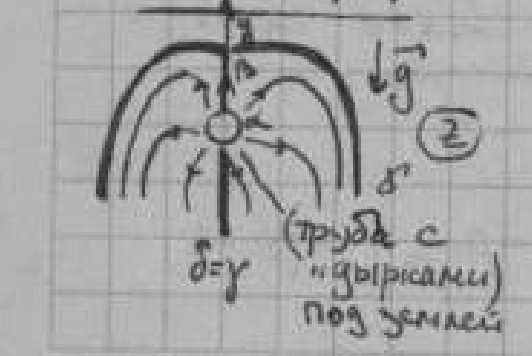
\includegraphics[width=.38\linewidth]{figures/notes-physical-domain.png}
\hspace{.04\linewidth}
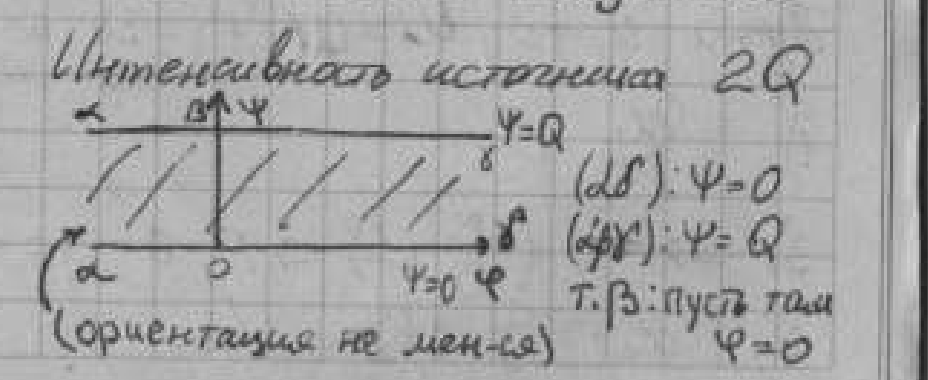
\includegraphics[width=.54\linewidth]{figures/notes-potential-domain.png}
\end{center}
Труба с «дырками» под землей.

\[
(\alpha\delta):\ \psi=0,\qquad(\beta\gamma):\ \psi=Q.
\]
Т. $\beta$: пусть там $\varphi=0$.

(ориентация не мен-ся)

% Источник: porous-lecture-notes.pdf; печатная страница: неизвестна; страница файла: 15; видимый рукописный номер разворота: 15
\begin{center}
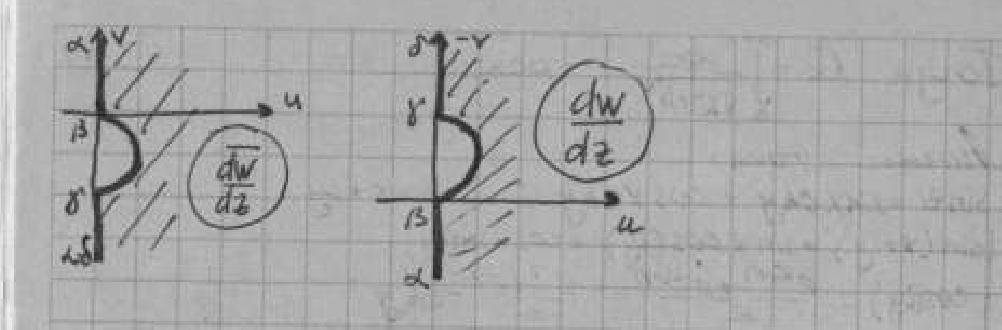
\includegraphics[width=.85\linewidth]{figures/notes-hodographs.png}
\end{center}
% На странице файла 15 включены только два рисунка-образа области течения, продолжающие постановку задачи на странице 14. Далее начинается «Гидравлическая теория ф-ции», не входящая в выбранный фрагмент.
